\documentclass{standalone}
\usepackage{mintikz}

\usepackage{xfp}

\begin{document}
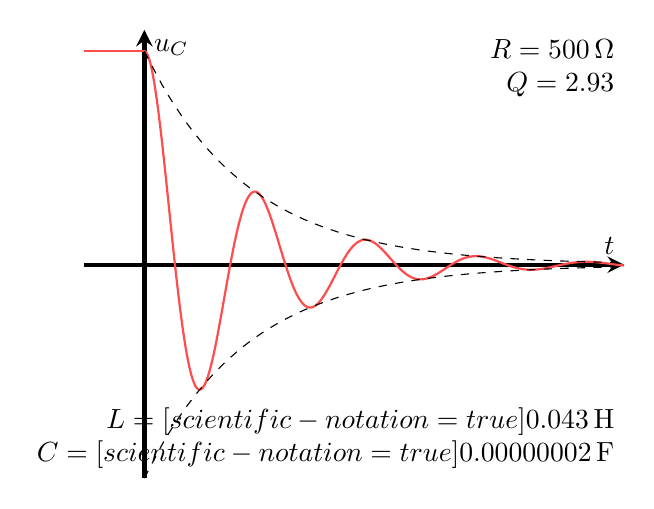
\begin{tikzpicture}[]
	\def\E{2}
	\def\R{500}
	\def\L{0.043}
	\def\C{0.00000002}
	\def\Q{(1/\R)*sqrt(\L/\C)}
	\def\wo{sqrt(1/(\L*\C))}
	\def\w{\wo*sqrt(1-1/(4*\Q^2))}
	\def\xmax{.8e-3}
	% \def\Q{14.66}
	% \def\wo{34100}
	% \def\w{\wo*sqrt(1-1/(4*\Q^2))}
	\begin{axis}[
			xmin=-1e-4, xmax=\xmax,
			ymin=-2, ymax=2.2,
			xlabel=$t$, ylabel=$u_C$,
			axis lines=center,
			axis line style=ultra thick,
			xtick=\empty, ytick=\empty,
			clip=false]
		\addplot[thick,
			domain=-1e-4:0,
			samples=500,
			Red!70]
		{\E};
		\addplot[thick,
			domain=0:\xmax,
			samples=500,
			Red!70]
		{\E*exp(-(\wo*\x)/(2*\Q))*(cos(\w*\x r)+(\wo/(2*\Q*\w))*sin(\w*\x r))};
		\addplot[
			domain=0:\xmax,
			smooth, dashed,
			black]
		{\E*exp(-\wo*\x/(2*\Q))};
		\addplot[
			domain=0:\xmax,
			smooth, dashed,
			black]
		{-\E*exp(-\wo*\x/(2*\Q))};

		\node[anchor=north east, align=right] (RQtext) at (axis cs: \xmax, \E.2) {
			$R = \R\,\Omega$\\
			$Q = \fpeval{round(\Q,2)}$
		};
		\node[anchor=south east, align=right] (LCtext) at (axis cs: \xmax,-\E) {
			$L = \num[scientific-notation=true]{\L}\,\rm H$\\
			$C = \num[scientific-notation=true]{\C}\,\rm F$
		};
	\end{axis}
\end{tikzpicture}
\end{document}
